\section{Integrating multimodal health data for clinical predictions}

\newcommand{\nn}[2]{
    \begin{tikzpicture}
        \node[fill=gray!80, minimum width=3cm, minimum height=2cm, rounded corners=0.1cm, text=white, draw=black, font=\systemfont, anchor=south, text depth=1.5cm] (#2) at (0, 0) {
            #1
        };


        \neuron{n20}{($ (#2.south) + (0, 0.75) + (-1*\vsep, -1*\vsep) $)}
        \neuron{n21}{($ (n20) + (0, \vsep) $)}
        \neuron{n22}{($ (n20) + (0, 2*\vsep) $)}

        \neuron{n30}{($ (n20) + (\hsep, 0.5*\vsep) $)}
        \neuron{n31}{($ (n20) + (\hsep, 1.5*\vsep) $)}

        \neuron{n40}{($ (n20) + (2*\hsep, \vsep) $)}

        \foreach \j in {0,...,2} {
            \draw[black, opacity=\edgeopacity] ($ (#2.south west) + (0, 0.75) $) -- (n2\j);
        }

        \foreach \j in {0,...,2} {
            \foreach \k in {0,...,1} {
                \draw[black, opacity=\edgeopacity] (n2\j) -- (n3\k);
            }
        }
        \draw[black, opacity=\edgeopacity] (n30) -- (n40);
        \draw[black, opacity=\edgeopacity] (n31) -- (n40);
        \draw[black, opacity=\edgeopacity] (n40) -- ($ (#2.south east) + (0, 0.75) $);
    \end{tikzpicture}
}

\begin{frame}{Late fusion: independent insights, combined decisions}
    \begin{tikzpicture}
        \node[draw=black] at (-7, -3.25) {};
        \node[draw=black] at (7, 3.25) {};

        \node[anchor=east, inner sep=0pt] (input2) at (-4, 2) {
            {\Huge{\emoji{spiral-notepad}}}
        };
        \node[anchor=east, inner sep=0pt, draw=black] (input) at (-4, -0.25) {
            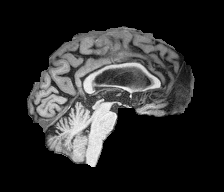
\includegraphics[width=1.5cm]{data/mri_sagittal.png}
        };
        \node[anchor=east, inner sep=0pt] (input3) at (-4, -2.5) {
            {\Huge{\emoji{microscope}}}
        };
        \only<2>{
            \node[] (ehr) at (-1, 2.25) {
                \nn{EHR-specific ANN}{ehrnn}
            };
            \node[anchor=west, font=\small] (output1) at (2, 1.99) {EHR-index};
            \draw[-stealth] (input2) -- ($ (ehr.west) - (-0.12, 0.26) $);
            \draw[-stealth] ($ (ehr.east) - (0.25, 0.26) $) -- (output1);
            \node[] (mri) at (-1, 0) {
                \nn{MRI-specific ANN}{mrinn}
            };
            \node[anchor=west, font=\small] (output2) at (2, -0.26) {MRI-index};
            \draw[-stealth] (input) -- ($ (mri.west) - (-0.12, 0.26) $);
            \draw[-stealth] ($ (mri.east) - (0.25, 0.26) $) -- (output2);
            \node[] (bio) at (-1, -2.25) {
                \nn{Bio-specific ANN}{bionn}
            };
            \node[anchor=west, font=\small] (output3) at (2, -2.51) {Bio-index};
            \draw[-stealth] (input3) -- ($ (bio.west) - (-0.12, 0.26) $);
            \draw[-stealth] ($ (bio.east) - (0.25, 0.26) $) -- (output3);

            \node[anchor=east, font=\small, align=left] (output) at (7, -0.26) {Clinical\\prediction};
            \draw[-stealth] (output1.east) -- (output);
            \draw[-stealth] (output2.east) -- (output);
            \draw[-stealth] (output3.east) -- (output);
        }
    \end{tikzpicture}
\end{frame}

\begin{frame}{Early fusion: blending information from the start}
    \begin{tikzpicture}
        \node[draw=black] at (-7, -3.25) {};
        \node[draw=black] at (7, 3.25) {};

        \node[fill=gray!80, minimum width=4cm, minimum height=2.9cm, rounded corners=0.1cm, text=white, draw=black, font=\systemfont, text depth=2.4cm, anchor=east] (ann) at (7, 0) {
            Modality-agnostic ANN
        };
        \only<1,3>{
            \neuron{n00}{($ (ann.south) + (0, 1.25) + (-2*\hsep, -2*\vsep) $)}
            \neuron{n01}{($ (n00) + (0, \vsep) $)}
            \neuron{n02}{($ (n00) + (0, 2*\vsep) $)}
            \neuron{n03}{($ (n00) + (0, 3*\vsep) $)}
            \neuron{n04}{($ (n00) + (0, 4*\vsep) $)}
        }
        \only<2>{
            \neuron[uioblue]{n00}{($ (ann.south) + (0, 1.25) + (-2*\hsep, -2*\vsep) $)}
            \neuron[uioblue]{n01}{($ (n00) + (0, \vsep) $)}
            \neuron[uiored]{n02}{($ (n00) + (0, 2*\vsep) $)}
            \neuron[uiored]{n03}{($ (n00) + (0, 3*\vsep) $)}
            \neuron[uioblue]{n04}{($ (n00) + (0, 4*\vsep) $)}
        }

        \only<1,3>{
            \neuron{n10}{($ (n00) + (\hsep, 0.5*\vsep) $)}
            \neuron{n11}{($ (n00) + (\hsep, 1.5*\vsep) $)}
            \neuron{n12}{($ (n00) + (\hsep, 2.5*\vsep) $)}
            \neuron{n13}{($ (n00) + (\hsep, 3.5*\vsep) $)}
        }
        \only<2>{
            \neuron[uiored]{n10}{($ (n00) + (\hsep, 0.5*\vsep) $)}
            \neuron[uiored]{n11}{($ (n00) + (\hsep, 1.5*\vsep) $)}
            \neuron[uioblue]{n12}{($ (n00) + (\hsep, 2.5*\vsep) $)}
            \neuron[uiored]{n13}{($ (n00) + (\hsep, 3.5*\vsep) $)}
        }

        \only<1,3>{
            \neuron{n20}{($ (n00) + (2*\hsep, \vsep) $)}
            \neuron{n21}{($ (n00) + (2*\hsep, 2*\vsep) $)}
            \neuron{n22}{($ (n00) + (2*\hsep, 3*\vsep) $)}
        }
        \only<2>{
            \neuron[uiored!60!uioblue]{n20}{($ (n00) + (2*\hsep, \vsep) $)}
            \neuron[uiored!75!uioblue]{n21}{($ (n00) + (2*\hsep, 2*\vsep) $)}
            \neuron[uioblue!75!uiored]{n22}{($ (n00) + (2*\hsep, 3*\vsep) $)}
        }

        \only<1>{
            \neuron{n30}{($ (n00) + (3*\hsep, 1.5*\vsep) $)}
            \neuron{n31}{($ (n00) + (3*\hsep, 2.5*\vsep) $)}
        }
        \only<2>{
            \neuron[uiored!50!uioblue]{n30}{($ (n00) + (3*\hsep, 1.5*\vsep) $)}
            \neuron[uiored!50!uioblue]{n31}{($ (n00) + (3*\hsep, 2.5*\vsep) $)}
        }
        \only<3>{
            \neuron{n30}{($ (n00) + (3*\hsep, 1.5*\vsep) $)}
            \neuron[yellow]{n31}{($ (n00) + (3*\hsep, 2.5*\vsep) $)}
        }

        \only<1,3>{
            \neuron{n40}{($ (n00) + (4*\hsep, 2*\vsep) $)}
        }
        \only<2>{
            \neuron[uiored!50!uioblue]{n40}{($ (n00) + (4*\hsep, 2*\vsep) $)}
        }

        \foreach \j in {0,...,4} {
            \draw[black, opacity=\edgeopacity] ($ (ann.west) - (0, 0.2175) $) -- (n0\j);
        }

        \foreach \j in {0,...,4} {
            \foreach \k in {0,...,3} {
                \draw[black, opacity=\edgeopacity] (n0\j) -- (n1\k);
            }
        }
        \foreach \j in {0,...,3} {
            \foreach \k in {0,...,2} {
                \draw[black, opacity=\edgeopacity] (n1\j) -- (n2\k);
            }
        }
        \foreach \j in {0,...,2} {
            \foreach \k in {0,...,1} {
                \draw[black, opacity=\edgeopacity] (n2\j) -- (n3\k);
            }
        }
        \draw[black, opacity=\edgeopacity] (n30) -- (n40);
        \draw[black, opacity=\edgeopacity] (n31) -- (n40);
        \draw[black, opacity=\edgeopacity] (n40) -- ($ (ann.south east) + (0, 1.25) $);

        \node[anchor=east, inner sep=0pt] (text) at ($ (ann.south) + (0, 1.25) + (-10, 1.5) $) {
            {\Huge{\emoji{spiral-notepad}}}
        };
        \node[draw=black, align=center, rounded corners=0.1cm, anchor=west, font=\small] (texttokenizer) at ($ (text.east) + (1, 0) $) {Text\\tokenizer};
        \only<1-2>{
            \node[font=\scriptsize, inner sep=1pt, draw=black, anchor=west, text depth=0] (texttoken1) at ($ (texttokenizer.east) + (1, 0) $) {The};
            \node[font=\scriptsize, inner sep=1pt, draw=black, anchor=west, text depth=0] (texttoken2) at ($ (texttoken1.east) + (0.1, 0) $) {patient};
            \node[font=\scriptsize, inner sep=1pt, draw=black, anchor=west, text depth=0] (texttoken3) at ($ (texttoken2.east) + (0.1, 0) $) {has};
        }
        \only<3>{
            \node[font=\scriptsize, inner sep=1pt, draw=black, text depth=0] (texttoken2) at ($ (texttoken1.west)!0.5!(texttoken3.east) $) {Spiderman};
        }
        \draw[dashed, uioblue, thick] ($ (texttoken1.north west) + (-0.1, 0.1) $) -- ($ (texttoken3.north east) + (0.1, 0.1) $) -- ($ (texttoken3.south east) + (0.1, -0.1) $) -- ($ (texttoken1.south west) + (-0.1, -0.1) $) -- cycle;
        \node[anchor=south, text=uioblue, font=\scriptsize, inner sep=0pt] at ($ (texttoken2.north) + (0, 0.2) $) {Text tokens};
        \draw[-stealth] (text) -- (texttokenizer);
        \draw[-stealth] (texttokenizer) -- ($ (texttoken1.west) - (0.1, 0) $);
        \draw[-stealth] ($ (texttoken3.east) + (0.1, 0) $) -| ($ (ann.south west) + (-1, 1.25) $) --  ($ (ann.south west) + (0, 1.25) $);

        \node[anchor=east, inner sep=0pt, draw=black] (mri) at ($ (ann.south) + (0, 1.25) + (-10, -1.5) $) {
            \only<1-2>{%
                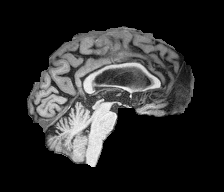
\includegraphics[width=1.5cm]{data/mri_sagittal.png}
            }%
            \only<3>{%
                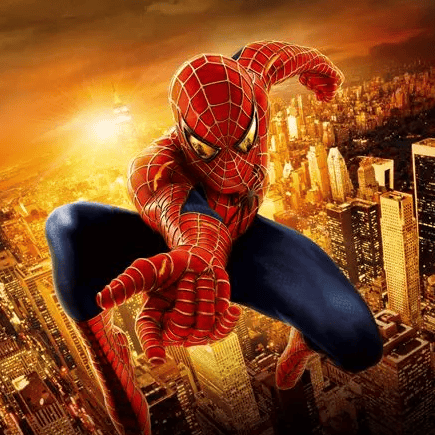
\includegraphics[width=1.5cm]{data/spiderman.png}
            }%
        };
        \node[draw=black, align=center, rounded corners=0.1cm, anchor=west, font=\small] (mritokenizer) at ($ (mri.east) + (1, 0) $) {Image\\tokenizer};
        \node[anchor=west, inner sep=0pt] (mritoken1) at ($ (mritokenizer.east) + (1, 0) $) {
            \only<1-2>{%
                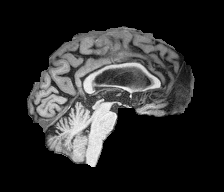
\includegraphics[
                    width=0.66cm,
                    trim={0cm 3.8cm 3.8cm 0cm},
                    clip
                ]{data/mri_sagittal.png}
            }%
            \only<3>{%
                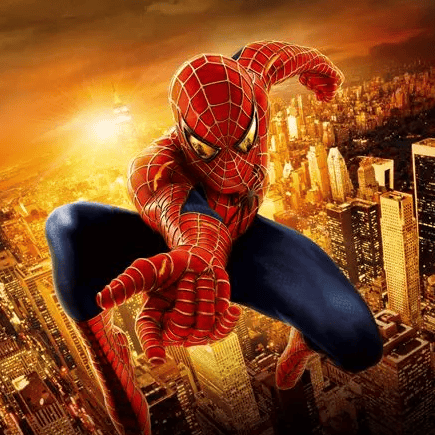
\includegraphics[
                    width=0.66cm,
                    trim={0cm 8cm 8cm 0cm},
                    clip
                ]{data/spiderman.png}
            }%
        };
        \node[anchor=west, inner sep=0pt] (mritoken2) at ($ (mritoken1.east) + (0.1, 0) $) {
            \only<1-2>{%
                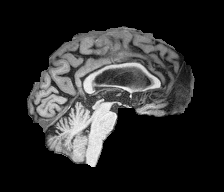
\includegraphics[
                    width=0.66cm,
                    trim={3.8cm 3.8cm 0cm 0cm},
                    clip
                ]{data/mri_sagittal.png}
            }%
            \only<3>{%
                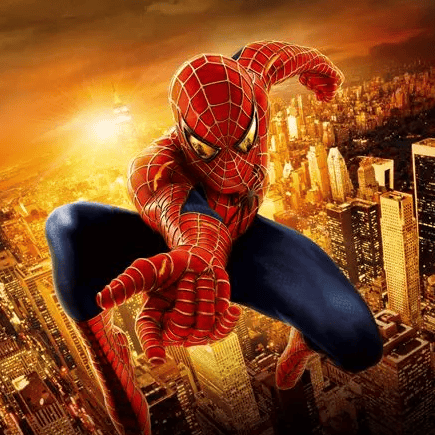
\includegraphics[
                    width=0.66cm,
                    trim={8cm 8cm 0cm 0cm},
                    clip
                ]{data/spiderman.png}
            }%
        };
        \node[anchor=west, inner sep=0pt] (mritoken3) at ($ (mritoken2.east) + (0.1, 0) $) {
            \only<1-2>{%
                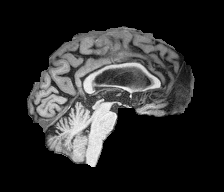
\includegraphics[
                    width=0.66cm,
                    trim={0cm 0cm 3.8cm 3.8cm},
                    clip
                ]{data/mri_sagittal.png}
            }%
            \only<3>{%
                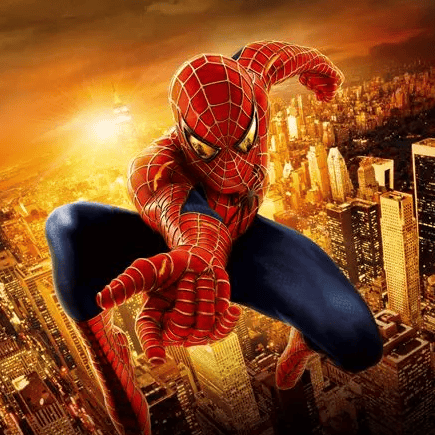
\includegraphics[
                    width=0.66cm,
                    trim={0cm 0cm 8cm 8cm},
                    clip
                ]{data/spiderman.png}
            }%
        };
        \draw[dashed, uiored, thick] ($ (mritoken1.north west) + (-0.1, 0.1) $) -- ($ (mritoken3.north east) + (0.1, 0.1) $) -- ($ (mritoken3.south east) + (0.1, -0.1) $) -- ($ (mritoken1.south west) + (-0.1, -0.1) $) -- cycle;
        \node[anchor=north, text=uiored, font=\scriptsize, inner sep=0pt] at ($ (mritoken2.south) - (0, 0.2) $) {Image tokens};

        \draw[-stealth] (mri) -- (mritokenizer);
        \draw[-stealth] (mritokenizer) -- ($ (mritoken1.west) - (0.1, 0) $);
        \draw[-stealth] ($ (mritoken3.east) + (0.1, 0) $) -| ($ (ann.south west) + (-1, 1.25) $) --  ($ (ann.south west) + (0, 1.25) $);


    \end{tikzpicture}
\end{frame}

\begin{frame}{Intermediate fusion: integrating insights along the way}
\end{frame}